\section{Introduction}
\cite{russakovsky2015imagenet} "In the last three years, mainly due to the advances of deep learning, more concretely convolutional
networks, the quality of image recognition and object detection has been progressing at a dramatic pace". \newline

However artificial NN are designed and fitted for single task, unlike human agents. \newline

\cite{DBLP:journals/corr/abs-1802-08195} "Goodfellow define adversarial examples as “inputs to machine learning models that an
attacker has intentionally designed to cause the model to make a mistake.” In the context of visual
object recognition, adversarial examples are images usually formed by applying a small perturbation
to a naturally occurring image in a way that breaks the predictions made by a machine learning
classifier". \newline

It’s widely known fact that NN are vulnerable against adversarial images. \newline
\cite{ilyas2019adversarial} "Particularly worrisome is the phenomenon of adversarial examples, imperceptibly perturbed natural inputs that induce erroneous predictions in state-of-the-art classifiers."\newline

The pretext task is the self-supervised learning task solved to learn visual representations, with the aim of using the learned representations or model weights obtained in the process, for the downstream task. \newline

\cite{kolesnikov2019revisiting} Pretext tasks had proven to increase models accuracy, and are also belived to contribute to model learning important (as per human agents) features. \newline

In this paper I would like to evaluate how state of art pretext tasks influence NN vulnerability against adversarial attacks.


\section{Background and Related work}

\subsection{Efficient Net}
Convultional networks' architectures for image recognition have evolved quite drastically in recent yers, with numerous options availabel "out of the box".
One which caught authors (my) eyes most recently was Efficient Net \cite{DBLP:journals/corr/abs-1905-11946} as it delivers impresive accuracy, while being able to scale better than a lot of others and being not so resource greedy.
So, I would be using it alogside with own way simpler implementation to evaluate the research. For the sake of \st{scientific} interest, I would use it in transfer learning manner, as well as train from scratch.

\subsection{Rotation pretext training}
\cite{kolesnikov2019revisiting} "Gidaris et al. propose to produce 4 copies of
a single image by rotating it by {0°, 90°, 180°, 270°} and let
a single network predict the rotation which was applied—a
4-class classification task. Intuitively, a good model should
learn to recognize canonical orientations of objects in natural images."

\subsection{Jigsaw pretext training}
Similar to approach described here \cite{kolesnikov2019revisiting},
the task is to recover relative spatial position of
4 randomly sampled image patches after a random permutation of these patches was performed.
All of these patches are concatenated in 'puzzle' image, which is later sent through same network, which needs to predict a permutation that
was used. In practice, all 24 possible permutations were used.

\subsection{Fast gradient sign method}
This name was first introduced in this paper \cite{goodfellow2015explaining} as guranteed approach to make artificial neural network missclassify image, which still would de be recognisable as of the same class for humans. \newline
The fast gradient sign method works by using the gradients of the neural network to create an adversarial example. For an input image, the method uses the gradients of the loss with respect to the input image to create a new image that maximises the loss. This new image is called the adversarial image. This can be summarised using the following expression: $adv\_x = x + \epsilon \cdot sign(\nabla_x J(\theta, x, y))$.


\section{Methods}

\subsection{Models}
The implementation was done using tensorflow framework using simple convultional network and EfficientNet alogside. Own basic implementation is based on \href{https://www.tensorflow.org/tutorials/images/classification}{Tensorflow image classification}.
For more details about EfficientNet usage, please refer to \href{https://keras.io/api/applications/efficientnet/}{Keras EfficientNet}.

\subsection{Pretext training}

\paragraph{Rotation}
Each image from original dataset was rotated 0°,90°,180°,270° and assigned new pseudo label in [0...3]. New images were shuffled then. The last dense layer of network was replaced with dense layer for corresponding number of pseudo classes (4). The same model was then trained to identify rotation applied.
\begin{figure}[!h]
    \begin{subfigure}{0.33\textwidth}
        \caption{Label = 0}
        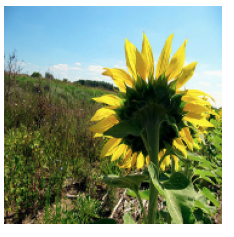
\includegraphics[width=5cm]{images/rot_0.png}
    \end{subfigure}
    \begin{subfigure}{0.2\textwidth}
        \caption{Label = 1}
        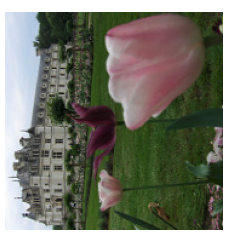
\includegraphics[width=5cm]{images/rot_1.png}
    \end{subfigure}
    \begin{subfigure}{0.33\textwidth}
        \caption{Label = 2}
        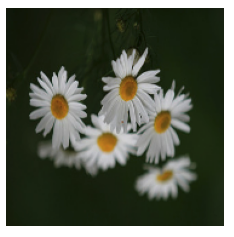
\includegraphics[width=5cm]{images/rot_2.png}
    \end{subfigure}
\end{figure}

\paragraph{Jigsaw}
For jigsaw I have addopted similar aproach as here \cite{DBLP:journals/corr/NorooziF16}.
Image was cut in 4 equal parts, which then have been permuted in all of 24 possible ways.
(number of possible permutation can be obtained from here $P=\frac{r!}{(r-n)!}$).
Similary to rotation pseudo labels in [0...23] have been assigned, data was shuffled and dense layer was replaced by suitable one.
The network then is learnt to identify which permutation was applied.

\begin{figure}[!h]
    \begin{subfigure}{0.33\textwidth}
        \caption{Original image}
        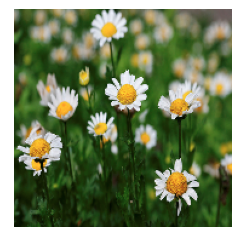
\includegraphics[width=5cm]{images/dandelion.png}
    \end{subfigure}
    \begin{subfigure}{0.2\textwidth}
        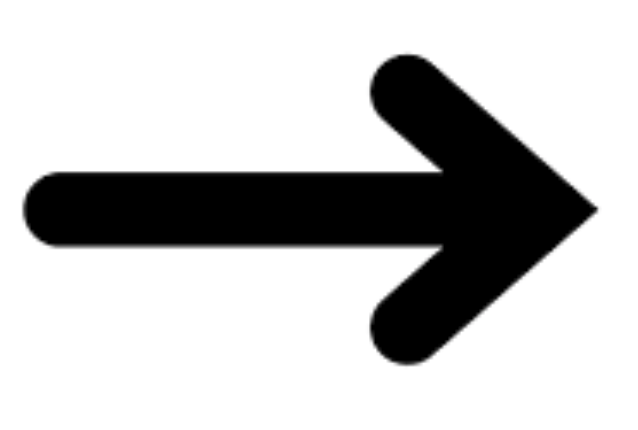
\includegraphics[width=3cm]{images/arrow.png}
    \end{subfigure}
    \begin{subfigure}{0.33\textwidth}
        \caption{Generated puzzle, with label=1}
        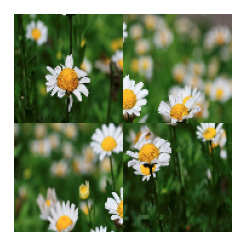
\includegraphics[width=5cm]{images/puzzle.png}
    \end{subfigure}
\end{figure}

\subsection{Adversarial Images with FGSM}
In order to addapt FGSM aproach described above, the gradient of loss this image's predictions generate is evaluated, multiplied with $\epsilon$ it results in perturbation, namely adversarial pattern for this image. Here is how it could look like:
\begin{figure}[!h]
    \begin{subfigure}{0.33\textwidth}
        \caption{Labrador retriever 41.82\% confidence}
        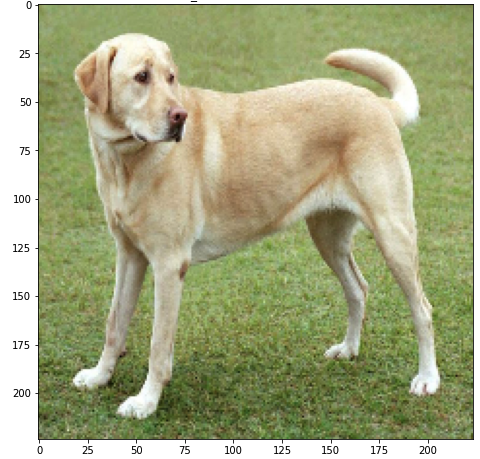
\includegraphics[width=5cm]{images/labrador.png}
    \end{subfigure}
    \begin{subfigure}{0.33\textwidth}
        \caption{Adversarial pattern}
        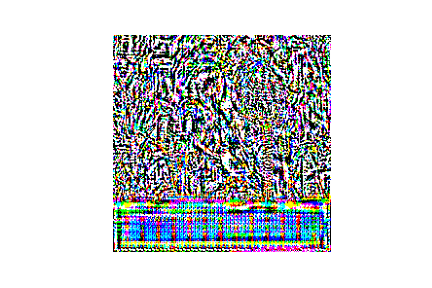
\includegraphics[width=5cm]{images/adv_pattern.png}
    \end{subfigure}
    \begin{subfigure}{0.3\textwidth}
        \caption{Weimaraner 15.13\% confidence}
        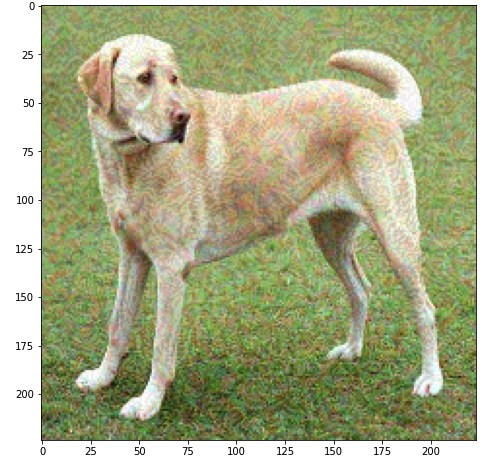
\includegraphics[width=5cm]{images/adv_labrador.png}
    \end{subfigure}
\end{figure}

\subsection{Evaluation approach}
In order to evaluate how including pretext task in training process influences NNs vulnerability against adversarial attacks, I have measured intensity of adversarial pattern needed to make NN missclassify
(Further denoted with epsilon or $\epsilon$).
\newline
5\% of dataset were reserved for experiment.
During each evaluation round NN network was trined with rotation or jigsaw, or both, or none pretext tasks. Number of training epochs was varied in [10, 20, 30, 50] for pretext and downstream task.
Reserved images were \st{fed} to NN, the ones, which were correctly classified saved.
Then each of saved (previously correctly classified images) was overlayed with adversarial pattern generated for it. $\epsilon$ was varied in [0.01, 0.1, 0.15], as any higher values cause image to be visually distrupted for human viewer.
The emprirical mean of smallest value needed to cause misslassification was saved.
$\overline{\epsilon}$ was compared for different values of pretext training epochs, downstream training epochs, and kinds of pretext tasks.